\documentclass[12pt]{article}

\usepackage{amssymb,amsmath,amsthm}
\usepackage{graphicx}
%\usepackage{fullpage}
\usepackage[final,colorlinks,hyperindex,unicode=true]{hyperref}
%\usepackage{tikz}
%\usepackage{pgfplots}
\usepackage[shadow,colorinlistoftodos,textwidth=3cm]{todonotes}
%\usepackage{fullpage}

%\newcommand{\jpgpic}[1]{\begin{center}\includegraphics[width=\textwidth]{#1.jpg}\end{center}}

\begin{document}
\author{M. Dvorkin, A. Kulikov}
%\title{A Bruijn Graph Approach}
%\title{Seeded assembly graph approach to {\it de novo} genome assembly}
\title{Earmark graph approach to {\it de novo} genome assembly}
\maketitle

%%%%%%%%%%%%%%%%%%%%%%%%%%%%%%%%%%%%%%%%%%%%%%%%%%%%%%%%%%%%%%%%%%%%%%%%%%%%%%%%%%%%%%%%%%%%%%%%%%%%%%%%%%%%%
\begin{abstract}
A common approach to assembling a genome from short reads is constructing
the de Bruijn graph on all $k$-mers from the given set of reads and finding a traversal of edges
in this graph. We propose a new approach that allows to decrease
the graph size without losing the essential information from the input data.
Instead of using all the $k$-mers from a read we take only a few of them
(and call them earmarked). Besides an obvious advantage of requiring less memory 
and time for constructing, the resulting earmark graph has several other advantages over the
de Bruijn graph. We discuss them in the paper and also present some experimental results.
\end{abstract}

%\listoftodos
\tableofcontents

%\newpage

%%%%%%%%%%%%%%%%%%%%%%%%%%%%%%%%%%%%%%%%%%%%%%%%%%%%%%%%%%%%%%%%%%%%%%%%%%%%%%%%%%%%%%%%%%%%%%%%%%%%%%%%%%%%%
\section{Introduction}
A common approach to assembling a genome from short reads is constructing
the de Bruijn graph \cite{PW01} on all $k$-mers from the given set of 
reads and finding a traversal of edges in this graph.
%Namely, the set of all $k$-mers form the set of vertices of the graph
%and two $k$-mers $A$ and $B$ are joined by a directed edge if there is a read
%where the $k$-mer $B$ appears 
An example of the de Bruijn graph for $k=3$ and a set of all reads of length $6$
of a (circular) genome $g={\tt ATGCATTGCACTGCA}$ is given in Fig.~\ref{fig:debruijn}a
(edges multiplicities are not shown). The genome spells an Eulerian
cycle in the de Bruijn graph.

\begin{figure}
\caption{(a) The de Bruijn graph built on $3$-mers 
of all $6$-reads of a toy genome {\tt ATGCATTGCACTGCA}.
(b) The earmark graph build on the same set of reads with all $3$-mers earmarked except for
{\tt TGC} and {\tt GCA}.}\label{fig:debruijn}
\begin{center}
a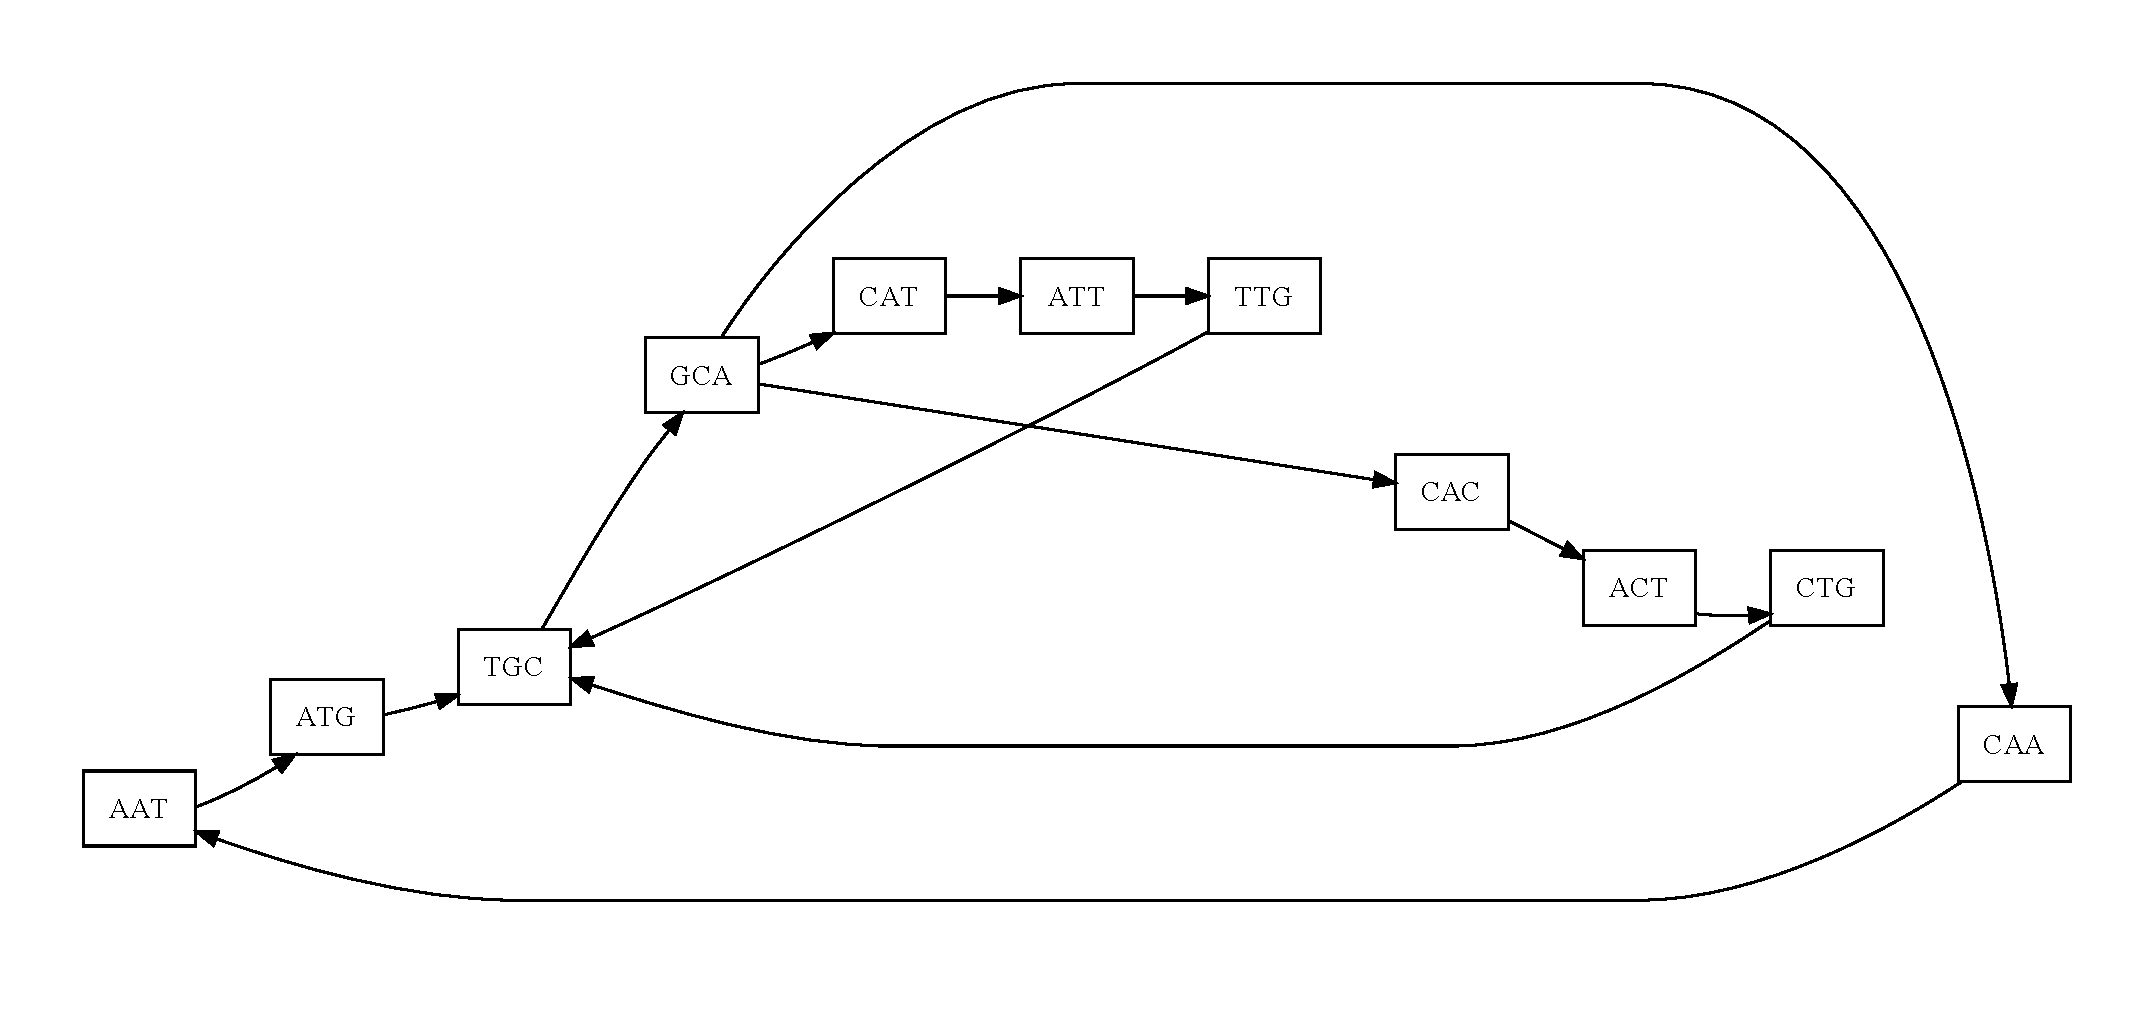
\includegraphics[width=0.9\textwidth]{ATGCATTGCACTGCA_debruijn.pdf}\\
b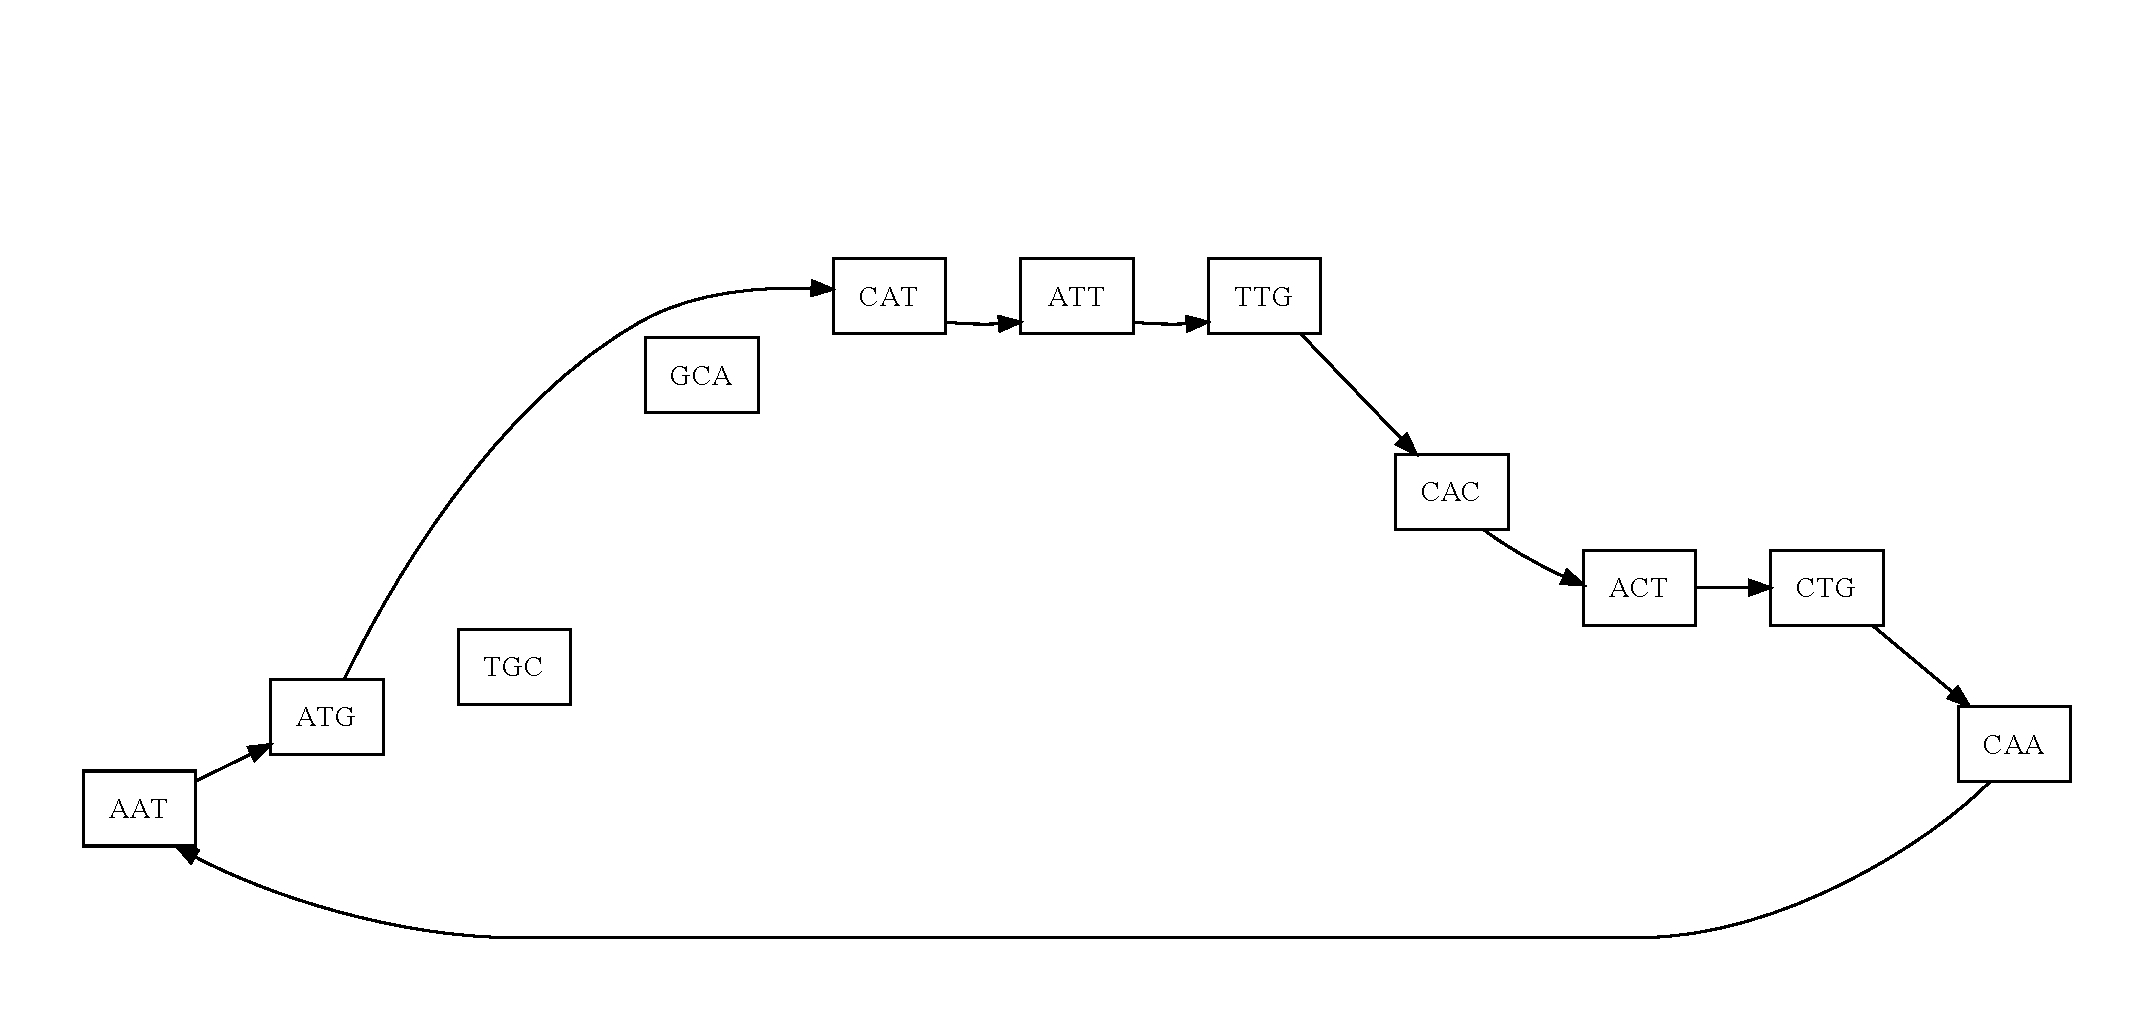
\includegraphics[width=0.9\textwidth]{ATGCATTGCACTGCA_earmark.pdf}\\
%\includegraphics[width=0.9\textwidth]{ATGCATTGCACTGCA_earmark2.pdf}\\
\end{center}
\end{figure}

\todo[inline]{explain why do we mark hash-values but nor k-mers}

The size of the de Bruijn graph for most genomes is huge making
it difficult to process. 
We propose a new approach that allows to decrease
the graph size without losing the essential information from the input data.
Instead of using all the $k$-mers from a read we take only some fraction of them
(and call them \emph{earmarked}).
Namely, instead 
of representing each read as a sequence of edges 
between its consecutive $k$-mers (in which case a read of length $r$ defines
$r-k-1$ edges) we represent it as just one (or a few, in general)
edge between some of its $k$-mers. For example, for 
reads {\tt ACGTACT} and {\tt TACTAGC} and $k=3$
instead of all gray edges in the figure below we will have 
only two black edges joining earmarked $k$-mers {\tt ACG}, {\tt ACT}, and {\tt AGC}.{\todo{redraw pictues in tikz
in the final version}}
\begin{center}
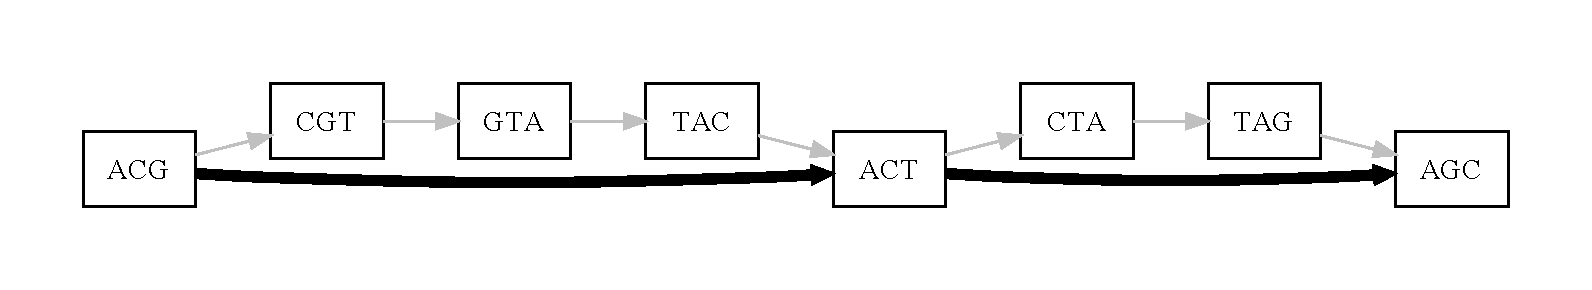
\includegraphics[width=0.9\textwidth]{fig1.pdf}
\end{center}
We call the resulting graph built on earmarked $k$-mers \emph{an earmark graph}.
It is a special case of the A-Bruijn graph introduced by Pevzner, Tang, and Tesler \cite{PTG04}.
An example of the earmark graph for the same genome $g={\tt ATGCATTGCACTGCA}$ is shown in Fig.~\ref{fig:debruijn}b.
Here, all $3$-mers are earmarked except for {\tt TGC} and {\tt GCA}.
Besides an obvious advantage of requiring less memory 
and time for constructing, the resulting earmark graph has several other advantages over the
de Bruijn graph. We discuss them after all the necessary definitions.

Our approach is inspired by the work by Roberts et al. \cite{RW04} on sequence comparison.
The problem they studied is a pairwise comparison of a set of strings. 
One of the approaches to this problem is the seed-and-extend approach.
One first stores the set of all possible $k$-mers from a given set of strings.
Then, only pairs of strings that both have the same $k$-mer as a substring are compared.
This allows to avoid comparing all pairs of input strings. However the database
of all $k$-mers may be really huge. To reduce the storage requirements Roberts et al. propose
to select not all the $k$-mers, but only those that are minimal in an input string with respect
to a certain order. Such $k$-mers are called \emph{minimizers}. Our earmarked $k$-mers are close in spirit 
to these minimizers.

%%%%%%%%%%%%%%%%%%%%%%%%%%%%%%%%%%%%%%%%%%%%%%%%%%%%%%%%%%%%%%%%%%%%%%%%%%%%%%%%%%%%%%%%%%%%%%%%%%%%%%%%%%%%%
\section{Earmark graph}

Let $0<k<r$ be integers and ${\cal R} \subseteq \{A,C,G,T\}^r$ be a set of reads
of length $r$. For a read $R$ and indices $1 \le i \le j \le r$,
let $R[i,j]$ be a substring of $R$ starting at position $i$
and ending at position $j$.
A \emph{de Bruijn graph} $\textrm{DG}_k({\cal R})$ is defined as follows:
\begin{itemize}
\item the set of all substrings of length $k$ (or just $k$-mers) of the given reads is the 
set of vertices; 
\item two $k$-mers $A$ and $B$ are joined by a directed edge if there is a
read $R \in {\cal R}$ and an index $1 \le i \le r-k-1$ such that
%$A$ and $B$ are substrings of $R$ starting at positions $i$ and $i+1$, respectively 
$A=R[i,i+k-1]$ and $B=R[i+1,i+k]$
(this, in particular, implies that
the suffix of $A$ of length $k-1$ equals the prefix of $B$ of the same length).{\todo{we should
take care about edges multiplicity here if we would like to speak about an Eulerian cycle
in this graph}}
\end{itemize}
Note that each read $R \in {\cal R}$ is represented by a path of length $r-k-1$
on its $k$-mers in $\textrm{DG}_k({\cal R})$.{\todo{tell that a genome corresponds to a cycle in this graph?..}}

An earmark graph can be viewed as the de Bruijn graph
with some paths contracted into a single edge.
Let ${\cal E} \subseteq \{A,C,G,T\}^k$ be a set of $k$-mers.
Below we refer to it as a \emph{set of earmarks} or as a \emph{set of earmarked $k$-mers}. 
An \emph{earmark graph} $\textrm{EG}_k({\cal R}, {\cal E})$ is defined as follows:
\begin{itemize}
\item ${\cal E}$ is the set of vertices;
\item two $k$-mers $A$ and $B$ are joined by a directed edge if there is a read $R \in {\cal R}$
and indices $1 \le i < j \le r-k-1$ such that
$A=R[i,i+k-1]$ and $B=R[j,j+k-1]$ and 
for any $i < t < j$, $R[t,t+k-1] \not \in {\cal E}$
(i.e., $B$ is the next earmarked $k$-mer after $A$ in $R$); the weight of this edge is set to
$j-i$.
\end{itemize}
Hence, in the earmark graph each read is represented as a path (of length at most $r-k-1$) on its earmarked $k$-mers.
When constructing an earmark graph it is reasonable to ensure that each read contains at least two 
earmarked $k$-mers (so that the length of the corresponding path is at least one).
It is easy to see that in the special case when we all the possible $k$-mers are earmarked
the earmark graph coincides with the de Bruijn graph. 

Both de Bruijn and earmark graphs are built on a set of reads that can be viewed as a 
set of reads from an unknown genome. A natural way to build these two graphs on a genome
itself is to use the set of all its reads of a particular length. Namely, 
for a genome $S \in \{A,C,G,T\}^*$, define $\Gamma_r(S) \subseteq \{A,C,G,T\}^r$
as a set of all $r$-mers appearing in $S$. Then $\textrm{DG}_k(S)$ and $\textrm{EG}_k(S, {\cal E})$
are just $\textrm{DG}_k(\Gamma_r(S))$ and $\textrm{EG}_k(\Gamma_r(S), {\cal E})$, respectively.

%This defintion can be used in a natural way to build the de Bruijn graph not on a set of reads,
%but on a genome. Namely, for a genome $S \in \{A,C,G,T\}^*$, define $\Gamma_r(S) \subseteq \{A,C,G,T\}^k$
%as a set of all $r$-mers appearing in $S$. Then, $\textrm{DB}()$

%%%%%%%%%%%%%%%%%%%%%%%%%%%%%%%%%%%%%%%%%%%%%%%%%%%%%%%%%%%%%%%%%%%%%%%%%%%%%%%%%%%%%%%%%%%%%%%%%%%%%%%%%%%%%
%\section{Selection of earmarks}
%In this section, we discuss 


%%%%%%%%%%%%%%%%%%%%%%%%%%%%%%%%%%%%%%%%%%%%%%%%%%%%%%%%%%%%%%%%%%%%%%%%%%%%%%%%%%%%%%%%%%%%%%%%%%%%%%%%%%%%%
\section{Earmark graph construction}
%In this section, we give a high-level description of the main parts of the assembler.
In this section, we give a high-level description of an earmark graph construction procedure.
When the graph is constructed we simplify it using methods similar to the ones used in
EULER and Velvet.{\todo{is it ok to give just one sentence about graph simplification here?}}

We first construct an initial set of earmarks and then extend it to reduce the number of tips
in the resulting graph. 

\subsection{Earmarks selection procedure}
To construct an initial set of earmarks ${\cal E}$, we select from each given read 
several $k$-mers that are minimial with respect to some ordering. Namely, 
let $h$ be a hash-function on the set of all possible $k$-mers and $t$ be a number.
We then select initial earmarks as follows.
%Iterative procedure for selecting the set of earmarked $k$-mers is the following:
\begin{enumerate}
\item For each read, select $t$ minimum hash values of its 
$k$-mers and add them to the global set of earmarked hash values.
\item If $t=1$, earmark the second smallest hash value for each read
with only one $k$-mer with earmarked hash value. This guarantees that each read has at least
two $k$-mers with earmarked hash values.
\item Add to ${\cal E}$ all $k$-mers that have their hash values earmarked.
%In each read, select $k$-mers that have their hash values earmarked.
%For corresponding vertices in the resulting A Bruijn graph, add all pairwise edges, storing their lengths.
%\item For each $k$-mer that has no left or right neighbours, find a neighbour on the corresponding side
%that has the smallest hash value and earmark it.
%\item Repeat the previous step to minimize the number of neighbourless $k$-mers.
\end{enumerate}

%This procedure results with an A-Bruijn graph that is subject to further processing.

\subsection{Tip extension procedure}
Assume that we are given a set of reads ${\cal R}$ of an unknown genome $S$.
It is easy to see that parts of the genome $S$ that are not covered by any read
from ${\cal R}$ create vertices of in- or our-degree one in $\textrm{DG}_k({\cal R})$.
Such vertices are called \emph{tips}. At the same time, the earmark graph may contain
tips not only because of coverage gaps, but also tips resulting from a bad choice of the 
set of earmarks. To give an example,
%Due to the fact that not all the k-mers are represented in the A-Bruijn graph,
%some extra gaps can be unwillingly created.
consider a genome substring $ABCDE$, where $B$ and $D$ are earmarked $k$-mers.
If none of the reads in the input data contain the whole substring $BCD$, then vertices corresponding to
$B$ and $D$ will be tips in the earmark graph.
Meanwhile reads containing $ABC$ and $CDE$ may be present in the input data (and hence the whole considered
part is covered by reads), so these vertices must not be tips.
%thus it is an error of the approach
%to call this vertices tips and to introduce a gap here.

The tip extension procedure is suggested to handle this issue.
It consists of three steps that are repeated consequently until no possible tip extensions are present.
(Each steps demands reading the entire input data. It is possible to reduce the procedure to less than three
steps, but much more memory will be used in that case).

\begin{enumerate}
\item By processing all the reads, find out for each earmarked $k$-mer, whether we have seen any
earmarked $k$-mer to the left of it and to the right from it.
Those earmarked $k$-mers that do not have either left or right ``neighbours'' are called left and right tips,
respectively.
\item By processing all the reads, find the collection of all the non-earmarked $k$-mers that
are present (at least once) in a read to the left of a left tip, or to the right of the right tip.
Call them possible tip extensions.
\item By processing all the reads, for each possible tip extension, record whether there was
any earmarked $k$-mer to the left of it and to the right of it.
\end{enumerate}

Now that this information is collected, each tip is being extended with
a possible tip extension using the following rules (in the order preference).

\begin{enumerate}
\item Check if any of its possible tip extensions was already selected as an earmark
(as a tip extension for some previously processed tip, using rules 2 and 3 below).
If so, continue to the next tip.
\item Check if any of its possible tip extensions has both left and right neighbours.
We select this extension as an earmark and thus eliminate at least one undesirable tip.
\item Select as an earmark the possible tip extension that is most distant (in base pairs)
from the tip being proccesed. Doing this, we do not eliminate a tip but we extend it as far
as possible. This helps us not to lose information near the actual gaps (or the ends of actual scaffolds).
{\todo{probably it is reasonable to give an example here?}}
\end{enumerate}

If no new earmarked $k$-mers were introduced after this procedure, then stop, otherwise repeat the entire procedure.

%%%%%%%%%%%%%%%%%%%%%%%%%%%%%%%%%%%%%%%%%%%%%%%%%%%%%%%%%%%%%%%%%%%%%%%%%%%%%%%%%%%%%%%%%%%%%%%%%%%%%%%%%%%%%
\section{Practical results}
\todo[inline]{to be written}


%%%%%%%%%%%%%%%%%%%%%%%%%%%%%%%%%%%%%%%%%%%%%%%%%%%%%%%%%%%%%%%%%%%%%%%%%%%%%%%%%%%%%%%%%%%%%%%%%%%%%%%%%%%%%
\section{Discussion and further ideas}
\todo[inline]{to be written}

\subsection{Advantages of earmark graph over de Bruijn graph}
\todo[inline]{should it be here?}

\subsection{A more careful earmarks selection}

\todo[inline]{paired read info?}

%%%%%%%%%%%%%%%%%%%%%%%%%%%%%%%%%%%%%%%%%%%%%%%%%%%%%%%%%%%%%%%%%%%%%%%%%%%%%%%%%%%%%%%%%%%%%%%%%%%%%%%%%%%%%
\todo[inline]{clean up the references}
\bibliographystyle{alpha}
\bibliography{bib}

\end{document}

%%%%%%%%%%%%%%%%%%%%%%%%%%%%%%%%%%%%%%%%%%%%%%%%%%%%%%%%%%%%%%%%%%%%%%%%%%%%%%%%%%%%%%%%%%%%%%%%%%%%%%%%%%%%%
%%%%%%%%%%%%%%%%%%%%%%%%%%%%%%%%%%%%%%%%%%%%%%%%%%%%%%%%%%%%%%%%%%%%%%%%%%%%%%%%%%%%%%%%%%%%%%%%%%%%%%%%%%%%%
%%%%%%%%%%%%%%%%%%%%%%%%%%%%%%%%%%%%%%%%%%%%%%%%%%%%%%%%%%%%%%%%%%%%%%%%%%%%%%%%%%%%%%%%%%%%%%%%%%%%%%%%%%%%%
%%%%%%%%%%%%%%%%%%%%%%%%%%%%%%%%%%%%%%%%%%%%%%%%%%%%%%%%%%%%%%%%%%%%%%%%%%%%%%%%%%%%%%%%%%%%%%%%%%%%%%%%%%%%%
%%%%%%%%%%%%%%%%%%%%%%%%%%%%%%%%%%%%%%%%%%%%%%%%%%%%%%%%%%%%%%%%%%%%%%%%%%%%%%%%%%%%%%%%%%%%%%%%%%%%%%%%%%%%%
%%%%%%%%%%%%%%%%%%%%%%%%%%%%%%%%%%%%%%%%%%%%%%%%%%%%%%%%%%%%%%%%%%%%%%%%%%%%%%%%%%%%%%%%%%%%%%%%%%%%%%%%%%%%%
%%%%%%%%%%%%%%%%%%%%%%%%%%%%%%%%%%%%%%%%%%%%%%%%%%%%%%%%%%%%%%%%%%%%%%%%%%%%%%%%%%%%%%%%%%%%%%%%%%%%%%%%%%%%%


\subsection{Example}

\begin{figure}
\caption{De Bruijn (grey) and A Bruijn (black) graphs of genomes {\tt ACTGACTGTTGACACTG} ($readsize=9$, $k=5$)
and {\tt ATTGGTACATTGTGGTACGTACTGACT} ($readsize=11$, $k=5$).}\label{fig23}
\begin{center}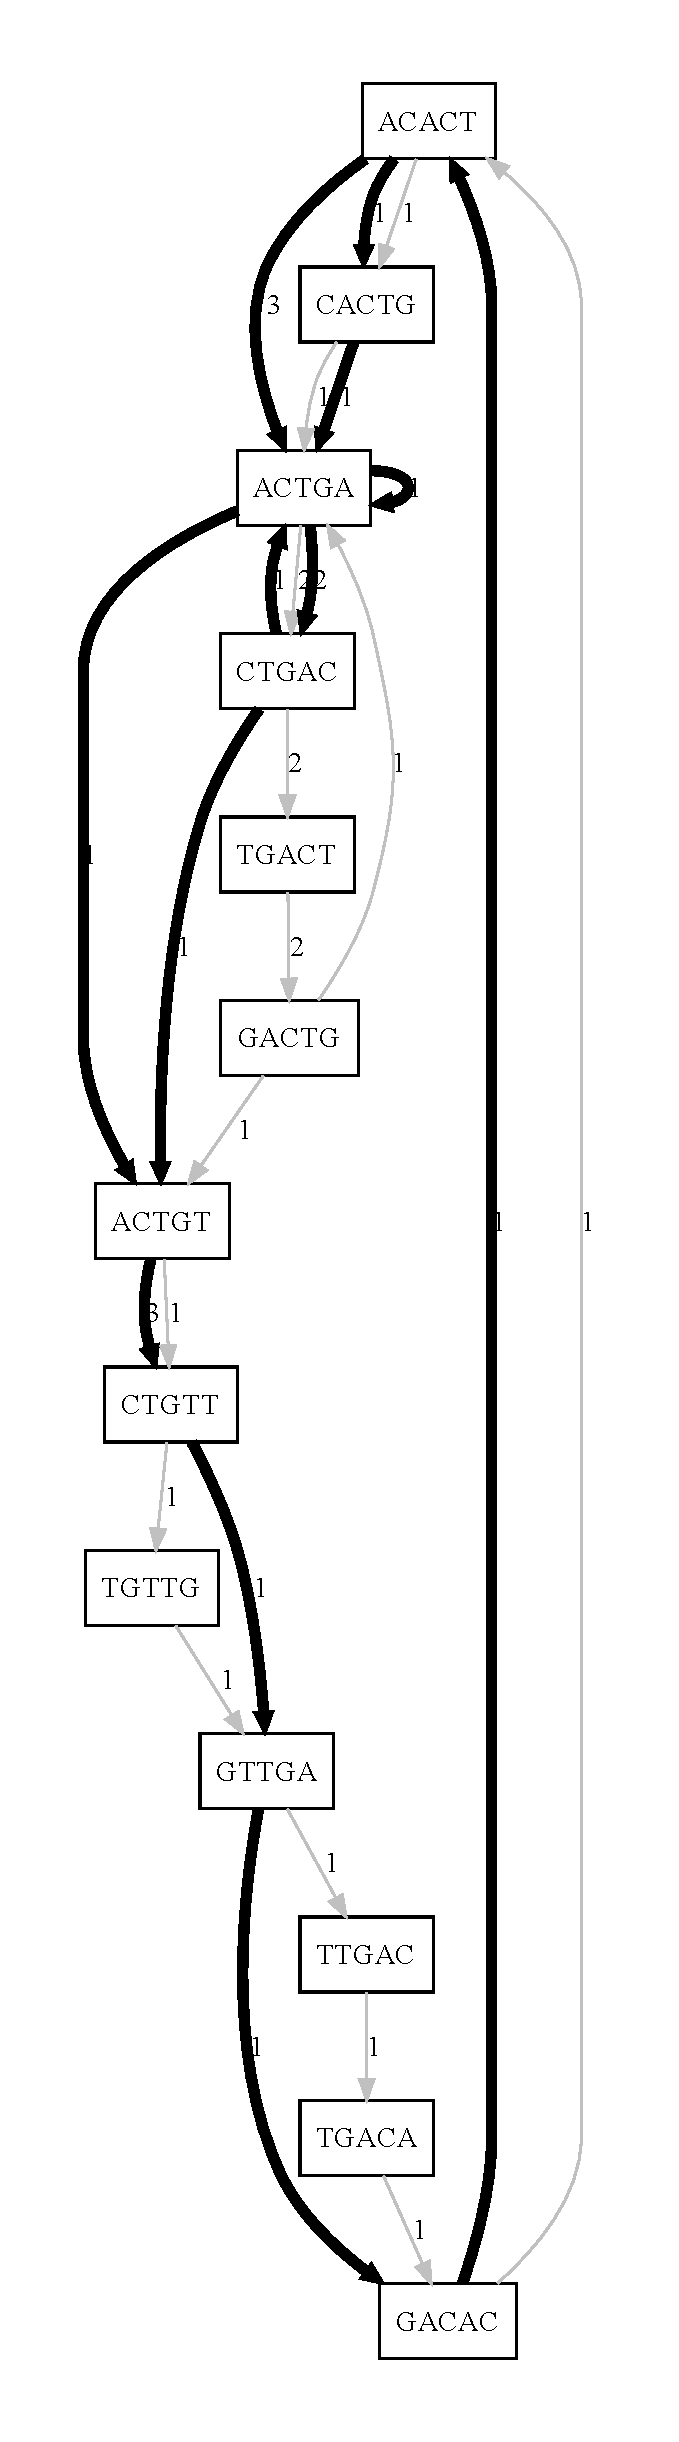
\includegraphics[height=0.9\textheight]{fig2.pdf}
~~~~~~~~~~~~~~
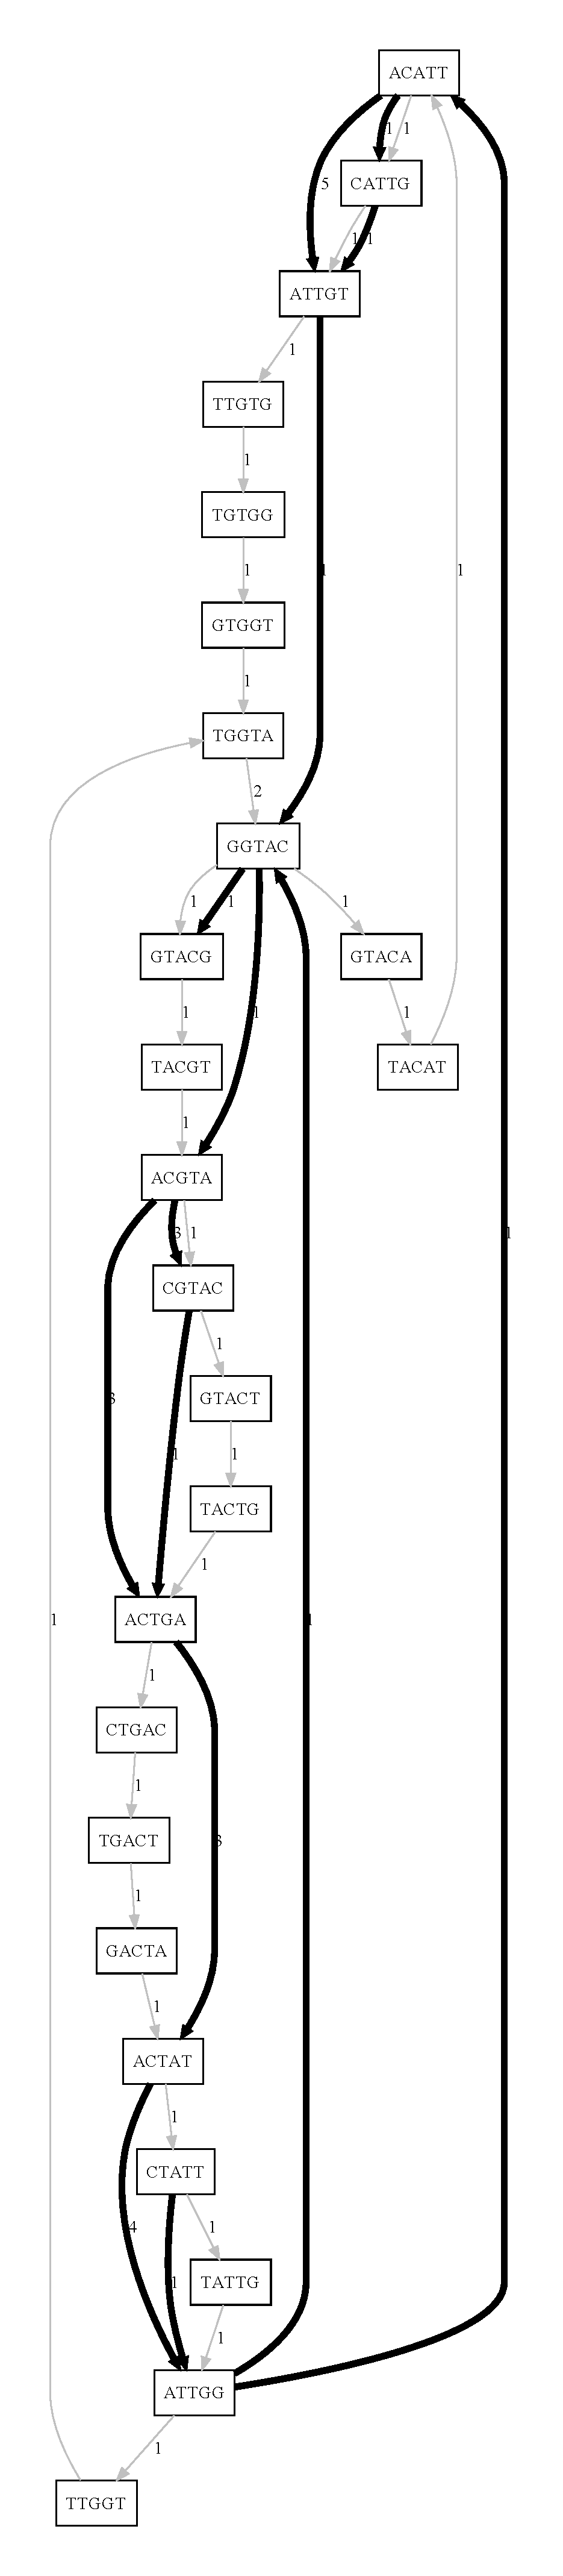
\includegraphics[height=0.9\textheight]{fig3.pdf}\end{center}
\end{figure}

Fig.~\ref{fig23} shows de Bruijn (black edges) and A Bruijn (grey edges) graphs for two toy genomes 
{\tt ACTGACTGTTGACACTG} and {\tt ATTGGTACATTGTGGTACGTACTGACT}. Numbers on edges are their multiplicities. 
We assume that the genome is circular and that we are given the set of all its reads.


\subsection{Advantages of A Bruijn graph over de Bruijn graph}
\begin{enumerate}
\item Clearly, it requires less memory.
\item In general, we expect that the resulting A Bruijn graph 
will have the same structure as the corresponding condensed de Bruijn graph.
If so, this would allow us to construct the condensed de Bruijn graph
using less time and memory.
\item If the used hash-function respects frequency of $k$-mers
the resulting graph will contain a smaller fraction of erroneous $k$-mers.
\item If the hash function does not mark $k$-mers that appear too often, then 
some of the repeats will be already resolved in A Bruijn graph.

An example of this effect is given in Fig.~\ref{fig:different_orderings}
where two A Bruijn graphs of a genome {\tt TAAACGAAAC} ($readsize=6$, $k=3$) 
are shown. The difference is in the way $3$-mers are ordered. Green edges 
correspond to the standard lexicographic ordering ({\tt AAA}$<${\tt 
AAC}$<\dots<${\tt TTT}). Now note that the considered genome contains a 
repeat {\tt AAAC}. Assume that the hash function treats $3$-mers {\tt AAA}
and {\tt AAC} from this repeat as maximal. Namely, let the ordering be the 
following:
\[{\tt TAA}<{\tt ACG}<{\tt CGA}<{\tt GAA}<{\tt CTA}<{\tt ACT}<{\tt AAA}<{\tt AAC} \, .\]
As figure shows, this ordering gives a graph consisting of just one cycle.
A slightly more complicated example is given on Fig.~\ref{fig:different_orderings2}.
There, the corresponding genome {\tt ATGCATTGCACTGCA} contains a repeat {\tt TGCA}
three times. Hence de Bruijn graph spells at least two different genomes. 
%By a careful choice of 


\begin{figure}
\caption{A Bruijn graphs of genome {\tt TAAACGAAAC} ($readsize=6$, $k=3$)
for different orderings on $3$-mers.}\label{fig:different_orderings}
\begin{center}
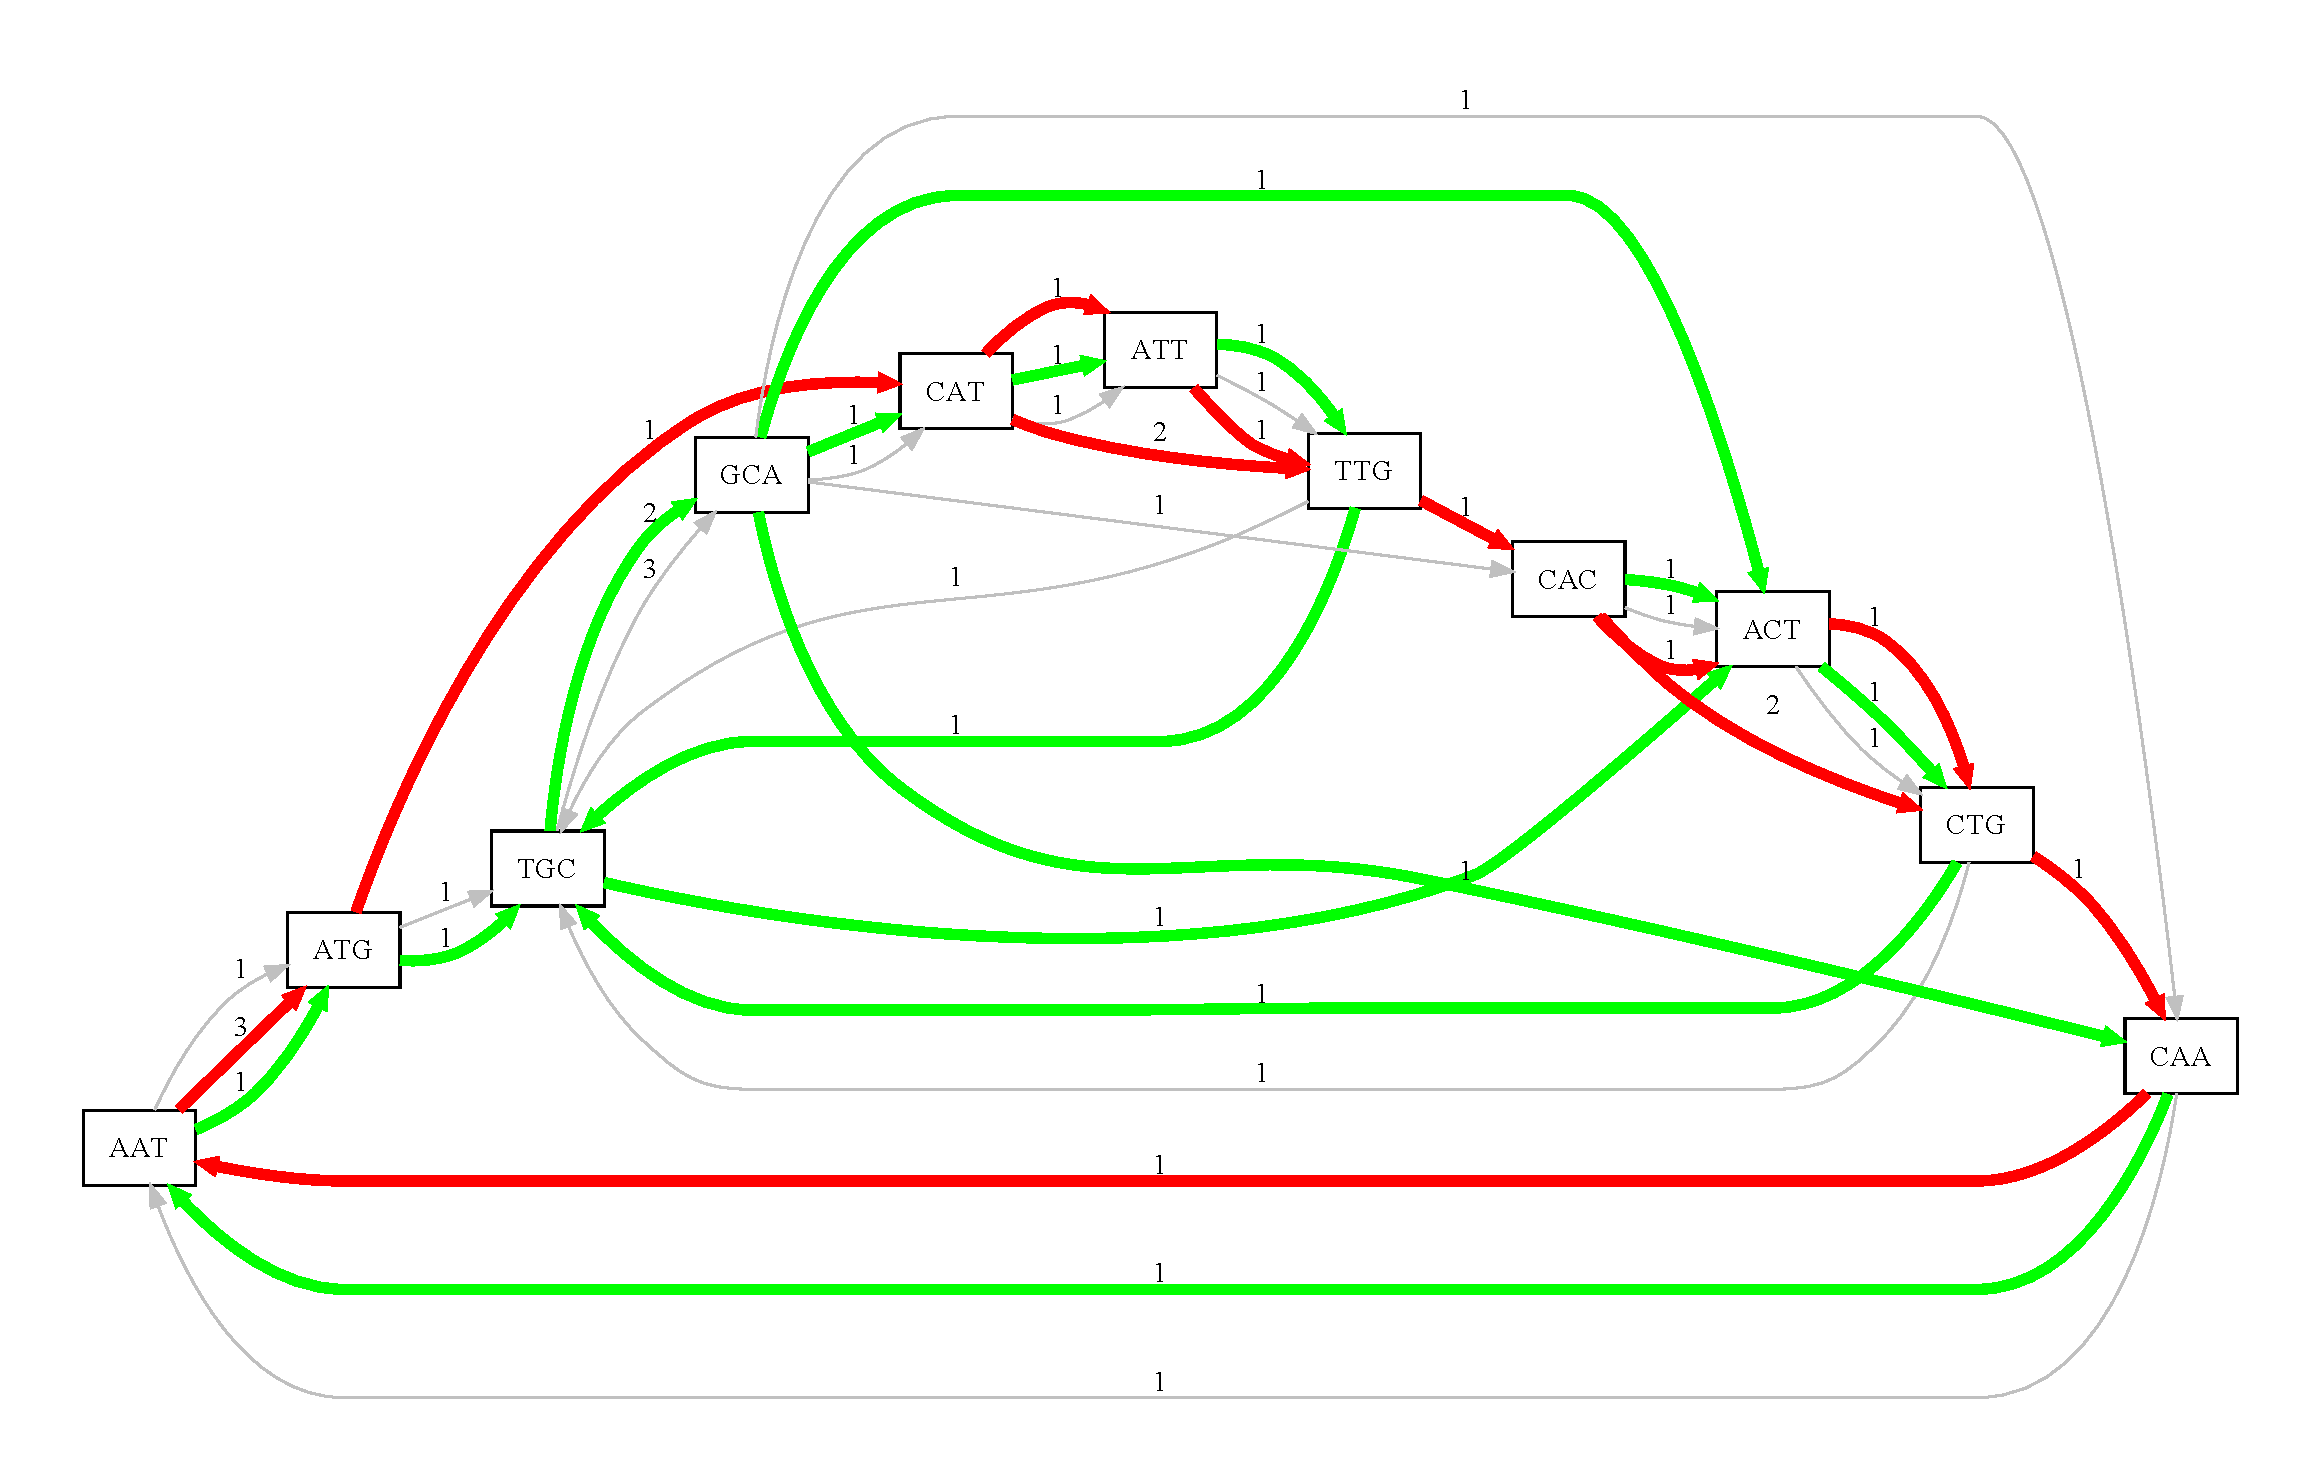
\includegraphics[width=0.9\textwidth]{TAAACGAAAC.pdf}
\end{center}
\end{figure}

\begin{figure}
\caption{A Bruijn graphs of genome {\tt ATGCATTGCACTGCA} ($readsize=6$, $k=3$)
for different orderings on $3$-mers.}\label{fig:different_orderings2}
\begin{center}
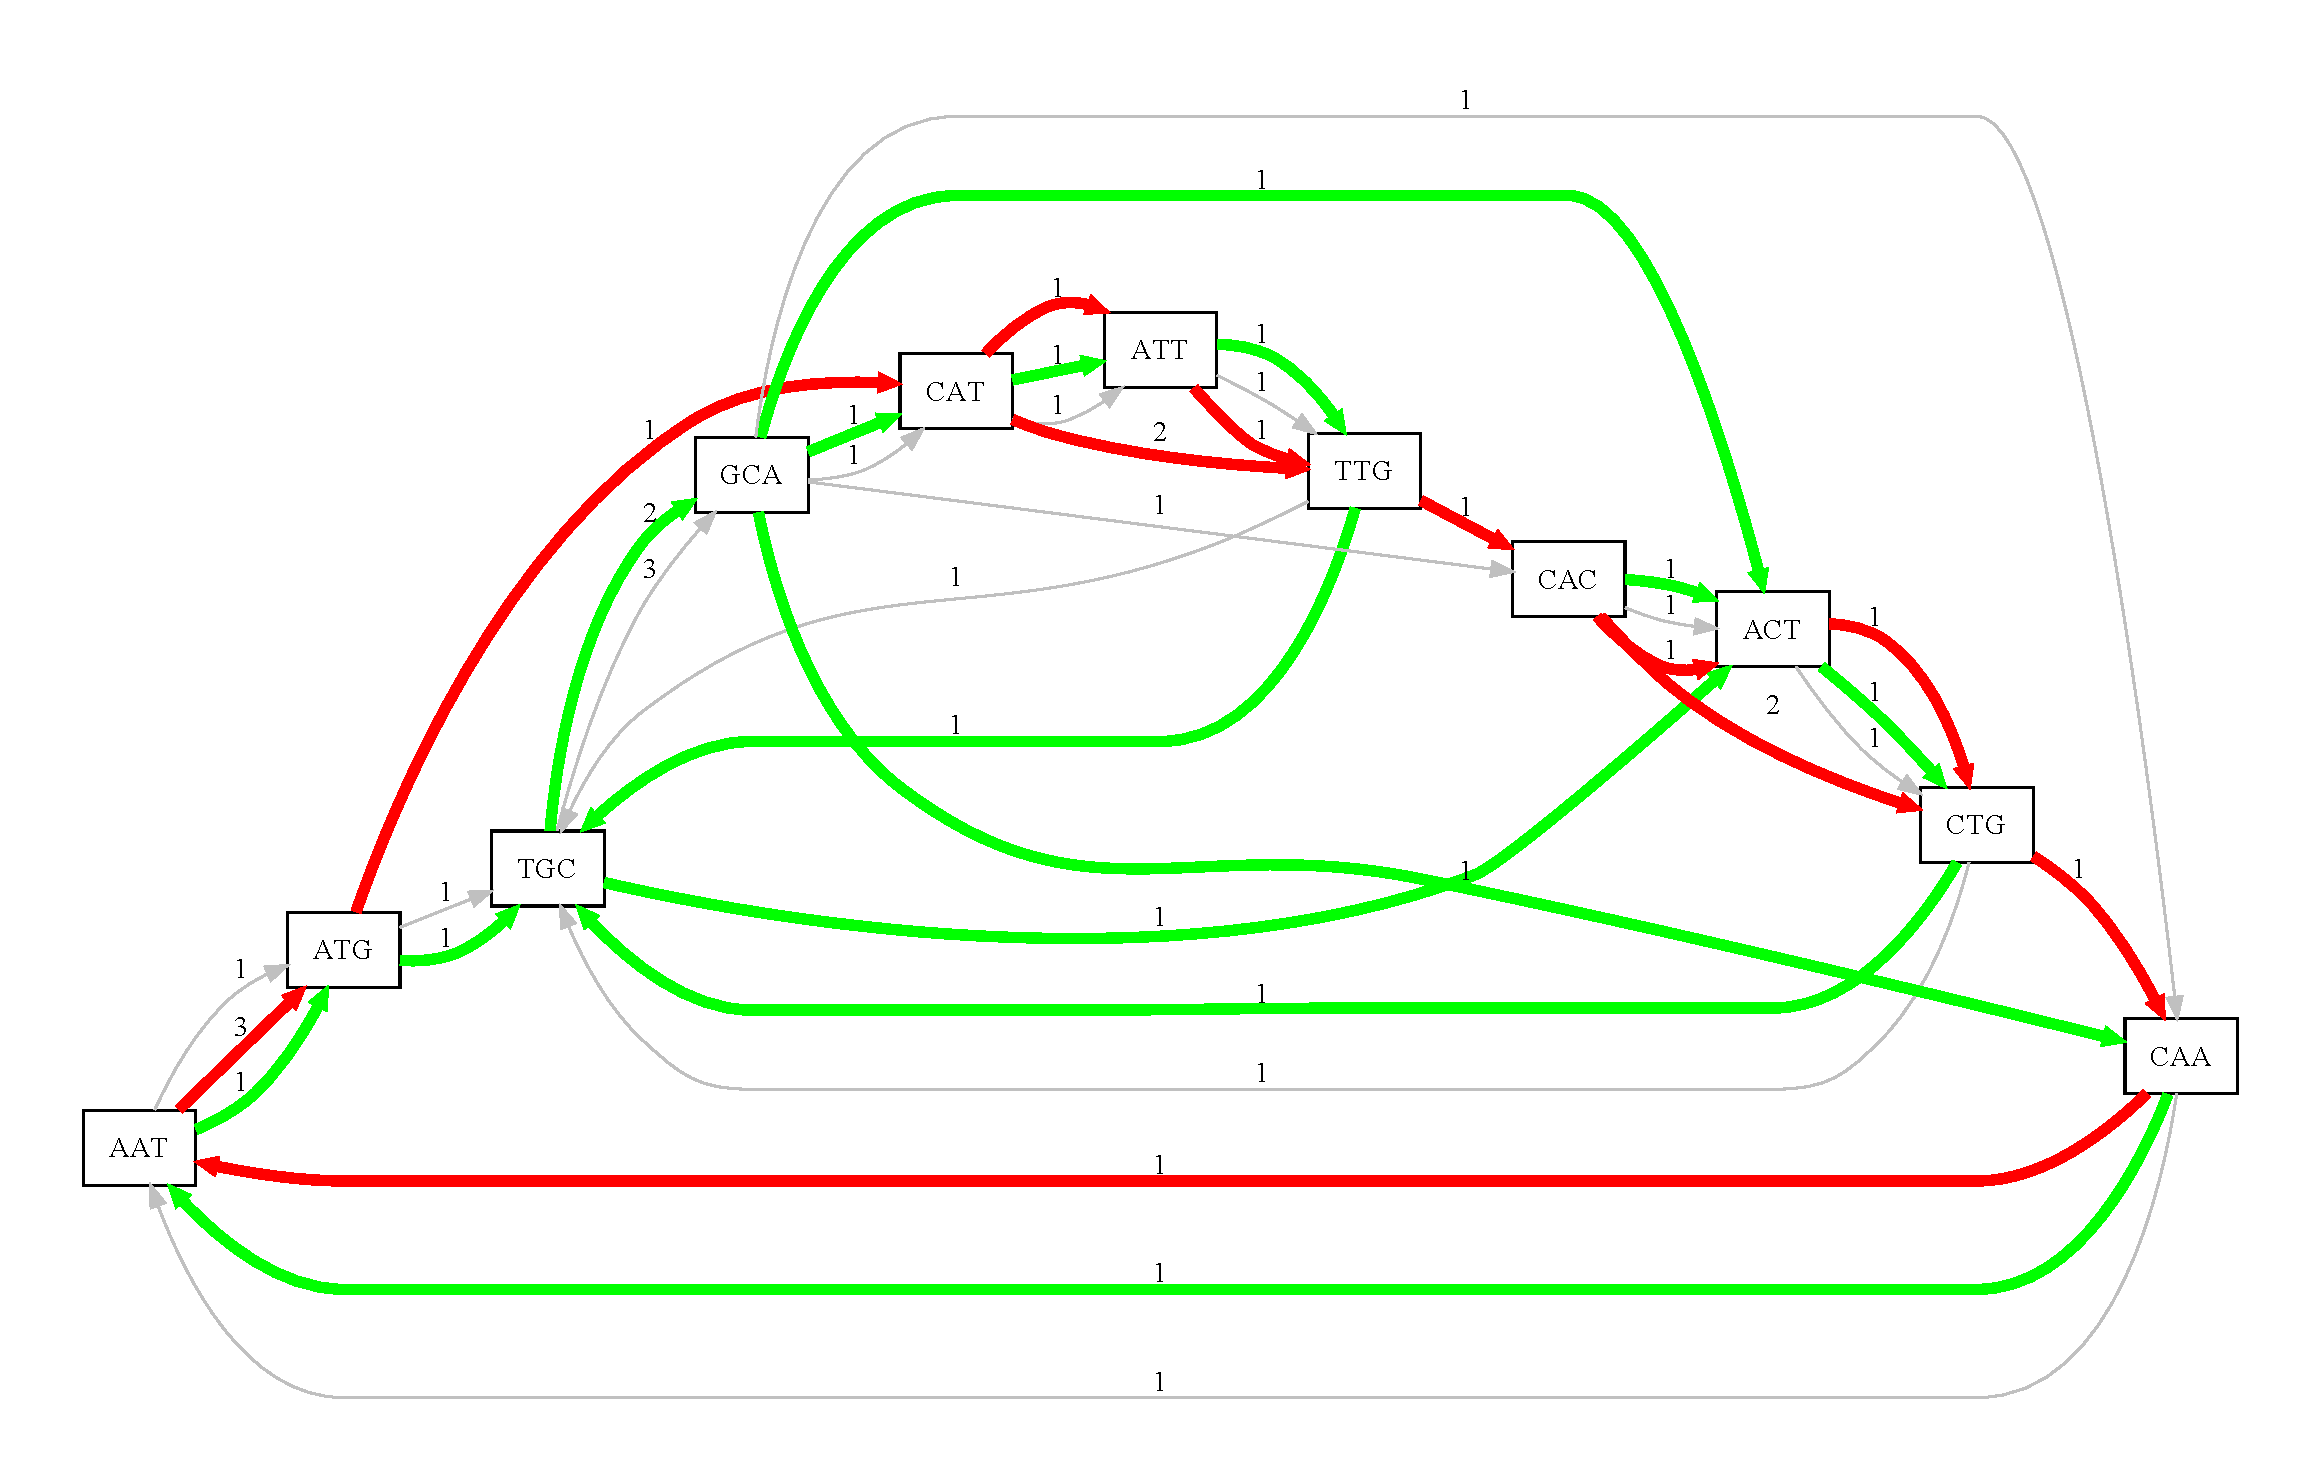
\includegraphics[width=0.9\textwidth]{ATGCATTGCACTGCA.pdf}
\end{center}
\end{figure}

\item \dots \todo{what else?..}
\end{enumerate}

\subsection{Hash Functions}

One of the possibilities to extract two distinguished $k$-mers out of a given
read is to take two $k$-mers with minimal value of some hash function $h$.
Some natural properties that $h$ should hold are listed below.
\begin{enumerate}
  \item The hash function should be easily computed.
  While iterating through all $k$-mers of a given read
  it is also important to have a fast way to recompute 
  the hash value. For this, one may take a kind of polynomial
  hash function (like in a finger-printing algorithm for the pattern 
  matching problem).
  \item It should to be stable with respect to reverse-complementary 
  $k$-mers, i.e., $h(s) = h(s^{RC})$ so that if we represent a read
  by an edge $(s_1,s_2)$, then its reverse-complement read is represented by 
  a ``reverse'' edge $(s_2^{RC},s_1^{RC})$. Two natural ways to make out a
  reverse-complementary stable hash function $h$ out of any hash function 
  $h_0$ are the following:
  \[h(s) = h_0(s) \oplus h_0(s^{RC}) \textrm{ or } h(s) = \min\{h_0(s), h_0(s^{RC})\} .\]
\end{enumerate}


The main question that still needs to be answered is:
does this graph really represent the repeat structure of the genome?

\section{Practical results}

We've implemented the suggested approach and are currently investigating the resulting A Bruijn graphs
on emulated data sets.

The technical issues pushed us towards a two-pass procedure:
\begin{enumerate}
  \item Each read undergoes a (linear-time) hashing procedure, and two least-valued $k$-mers are marked as
  ``good''. (In fact, not themselves but their hash values are marked. Even if a few extra $k$-mers become
  good due to hash collisions, it will not make much harm).
  \item For each read, all of its $k$-mers are checked whether their hash values are good, and the good ones
  are mapped to corresponding vertices in the future graph. The read is thus counted towards one or more edges.
  The leavings (in the two ends of the read) are currently not considered.
\end{enumerate}

Fig.~\ref{fig4} shows the resulting A Bruijn graph for the first 10\% of the reference E. Coli genome; the ideal data set
was used for this calculation.

\begin{figure}
\caption{10\% of E. Coli genome. $K$ = 31. Two $k$-mers from each read.}\label{fig4}
\begin{center}\includegraphics[height=0.9\textheight]{fig4.pdf}\end{center}
\end{figure}

This graph has only undergone a simple vertex-merging procedure; there are more
yet-unimplemented simplifications applicable to this graph.

\subsection{Statistics}
The plot below shows the dependence of the number of vertices in a graph from the 
number of reads for {\tt s\_6.first10000}.

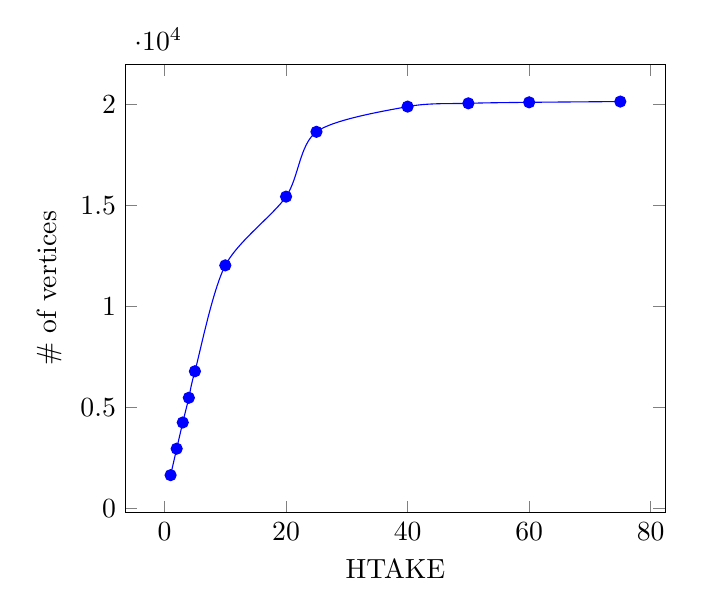
\begin{tikzpicture}
    \begin{axis}[xlabel={HTAKE},ylabel={$\#$ of vertices}]
    \addplot[smooth,mark=*,blue] plot coordinates { (1,1640) (2,2950) (3,4248) (4,5472) (5,6784)
      (10, 12028) (20, 15432) (25, 18642) (40, 19890) (50, 20052) (60, 20102) (75,20140) };
    %\addlegendentry{de Bruijn}
    \end{axis}
\end{tikzpicture}

The table below gives the number of vertices in a graph 
for two extreme values of {\tt HTAKE} (1 and 76) for {\tt s\_6.first10000}
(program version: Apr 25, 2011; $k=25$).


\begin{center}
\begin{tabular}{l|lll}
& \#bp=10000 & \#bp=100000 & \#bp=400000\\
\hline
${\tt HTAKE}=1$ & 1640 & 15916 & 62550\\
${\tt HTAKE}=76$ & 20144 & 202838 & 809730\\
ratio & $\approx 12.2$ & $\approx 12.7$ & $\approx 12.9$
\end{tabular}
\end{center}


\section{Further ideas}

\subsection{Making use of frequency}

The task of selecting the $k$-mers that will become vertices in the A Bruijn graph can be reformulated
as the task of selecting criteria that distinguish some $k$-mers among others that work the same way
in different reads.

Along with a hash function, an apt criterion is the frequency of the given $k$-mer among all reads
(provided the corresponding hash-table is memory-feasible). This criterion might be fruitful considering
the following.

\begin{itemize}
  \item The $k$-mers that are underrepresented
%  {\todo{what do we mean by ``underrepresented''?
%  is it true that most of the erroneous reads have frequency one?}}
  in the reads (even those a with small value of hash function)
  are (most probably) erroneous. Using frequency allows us 
  to exclude them from the set of
  vertex-forming $k$-mers.
  \item The $k$-mers that are overrepresented correspond to high-degree vertices in the graph.
  It might be helpful to exclude them as well in order to make the structure of the graph more feasible.
  (Motivation: consider two reads, $axyb$ and $cxyd$. A hash function might suggest to select $k$-mers $x$ and
  $y$ which would create a fork in the graph. Selecting $a$, $b$, $c$ and $d$ on the other hand leads to
  two separate edges.)
\end{itemize}

\subsection{Reducing the number of vertices}
As said in the beginning the main motivation for considering such graphs
is that they contain fewer edges than the original de Bruijn graph. Clearly, the number of edges in the
A Bruijn graph is also reduced (the vertices with no bold adjacent edges actually do not belong
to A Bruijn graph). In order to further reduce the number of vertices we can do the following.
First, mark just one $k$-mer in each read with the minimal possible hash value. If it turned out to be
the first or the last $k$-mer of the current read, mark one more $k$-mer with the next smallest hash 
value.

In the ideal case when each possible read is present in the set of reads, this guarantess that
at least two $k$-mers will be marked in each read.
In real situations it would be reasonable to take the second $k$-mer if the first one
falls into on of the leftmost or rightmost $\tau$ positions for some treshold $\tau$.

\subsection{Paired reads}

Each single read provides one or several edges with the information of the following kind:
the two end-vertices of this edge are likely to be present in the desired graph traversal
at the distance exactly $d$ from each other.

Meanwhile, paired reads provide the information of the similar kind, but with the distance
known approximately instead of exactly.
It is a question of a separate investigation whether the approximate distances known from
paired reads is helpful when traversing an A Bruijn graph.


\section{Pseudocode of the assembler}

\todo[inline]{add high-level description of the assembler}


%\section{Schedule}
%\begin{description}
%  \item[April 15] implement earmarking procedure
%  \item[April 18] test earmarking procedure on real data, get general statistics
%  \item[April 20] test different hashing parameters on real data
%  \item[April 22] implement frequency-dependent heuristics
%  \item[April 17] test graph condensation on real data
%  \item[April 30] research into the effects of different hash functions 
%  used to take minimizers
%  \item[May 10] compare the resulting A Bruijn graph with the condensed de 
%  Bruijn graph
%  \item 
%\end{description}

